\documentclass[10pt,xcolor=pdflatex]{beamer}
\usepackage{newcent}
\usepackage[utf8]{inputenc}
\usepackage[czech]{babel}
\usepackage{hyperref}
\usepackage{fancyvrb}
\usepackage{verbatim}
\usepackage{multirow}
%\usetheme[]{FIT}
\usetheme[CZlogo]{FIT} % CZ logo

%%%%%%%%%%%%%%%%%%%%%%%%%%%%%%%%%%%%%%%%%%%%%%%%%%%%%%%%%%%%%%%%%%
\title[]{Určení typu a směru zbraně v obrazové scéně}

\author[]{Róbert Kolcún}

%\institute[]{Brno University of Technology, Faculty of Information Technology\\
%Bo\v{z}et\v{e}chova 1/2. 612 66 Brno - Kr\'alovo Pole\\
%login@fit.vutbr.cz}

% CZ verzia
\institute[]{Vysoké učení technické v Brně, Fakulta informačních technologií\\
Božetěchova 1/2 612 66 Brno - Kr\'alovo Pole\\
xkolcu00@fit.vutbr.cz}


\date{8. Jún 2018}
%\date{\today}
%\date{} % bez data

%%%%%%%%%%%%%%%%%%%%%%%%%%%%%%%%%%%%%%%%%%%%%%%%%%%%%%%%%%%%%%%%%%

\begin{document}

\frame[plain]{\titlepage}

% Frame
\begin{frame}\frametitle{Cieľ práce}
    \begin{itemize}
        \item Klasifikácia zbraní do dvoch kategórií.
        \item Určenie náklonu zbrane v troch osách.
    \end{itemize}

    \begin{figure}[H]
        \centering
        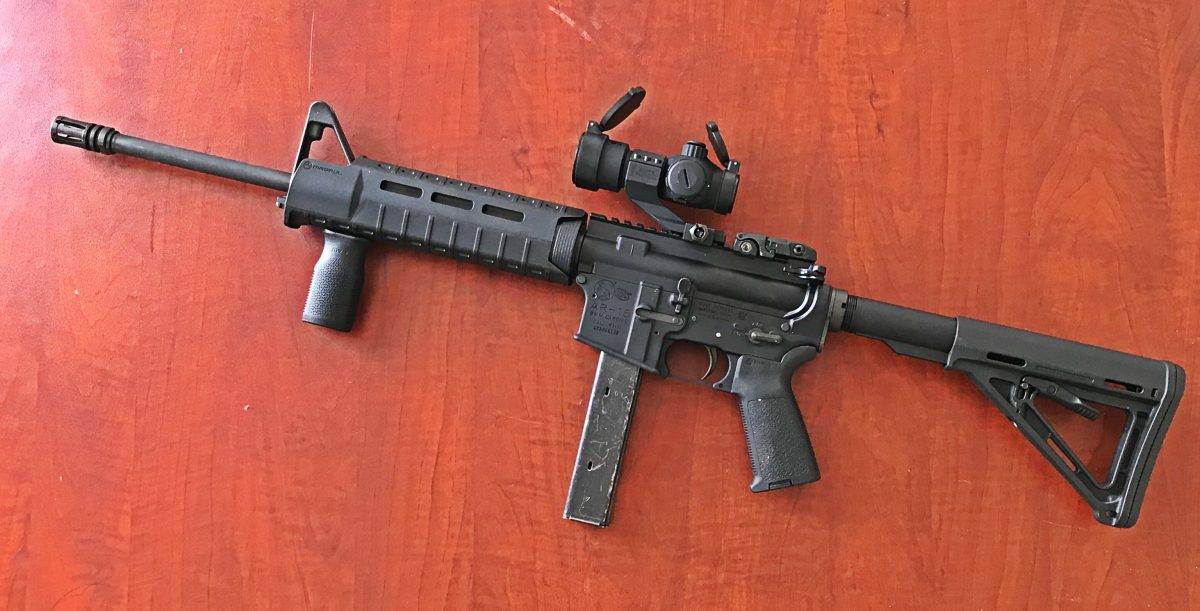
\includegraphics[width=0.5\textwidth]{img/long-weapon}
        \qquad
        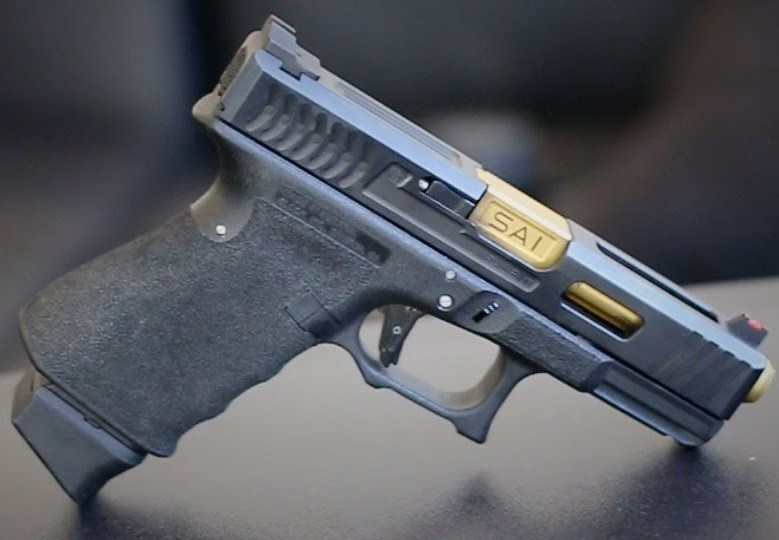
\includegraphics[width=0.4\textwidth]{img/short-weapon}
        \caption{Príklad vstupných dát.}
    \end{figure}

\end{frame}


% Frame
\begin{frame}\frametitle{Návrhovaný postup}
    \begin{itemize}
        \item Extrakcia príznakov a predspracovanie obrazu
        \begin{itemize}
            \item Histogram of Oriented Gradients

            \begin{figure}[H]
                \centering
                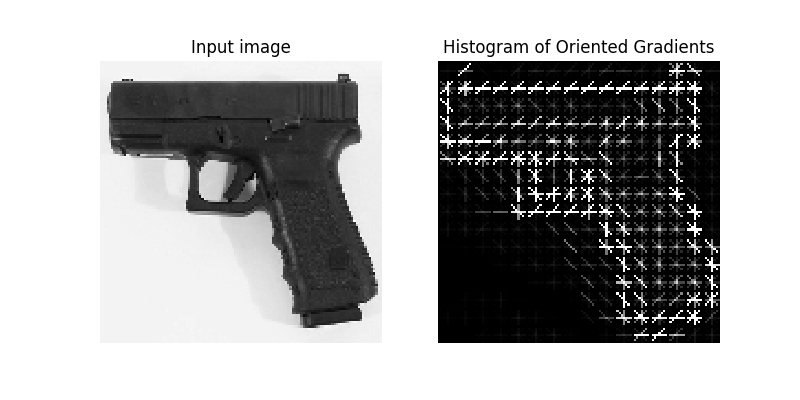
\includegraphics[width=0.55\textwidth]{img/hog}
                \caption{Príklad exktrakcie príznakov.}
            \end{figure}

            \item Augmentácia dát

            \begin{figure}[H]
                \centering
                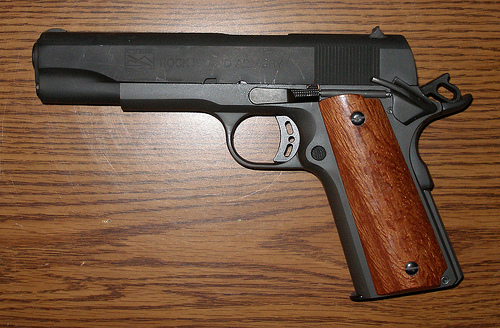
\includegraphics[width=0.3\textwidth]{img/weapon}
                \qquad
                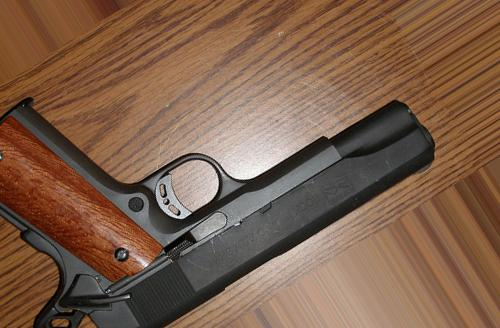
\includegraphics[width=0.30\textwidth]{img/weapon-augmented}
                \caption{Originálny obrázok(vľavo), augmentovaný obrázok(vpravo).}
            \end{figure}
        \end{itemize}
    \end{itemize}
\end{frame}

% Frame
\begin{frame}\frametitle{Klasifikácia typu zbrane}
    \begin{itemize}
        \item 2 kategórie - krátke a dlhé
        \vspace{0.3cm}
        \item Klasický prístup - SVM, K-Nearest-Neighbour
        \vspace{0.1cm}
        \item Konvolučné neurónové siete - 2 architektúry (AlexNetLike, VGGLike)
    \end{itemize}
\end{frame}

\begin{frame}\frametitle{Určenie náklonu zbrane}
    \begin{itemize}
        \item Klasifikácia do 72 kategórií po 5 stupňov.
        \item Tri modely - tri osi.
        \vspace{0.2cm}
        \item Konvolučné neurónové siete - 2 architektúry (AlexNetLike, VGGLike)
    \end{itemize}

    \begin{figure}[H]
        \centering
        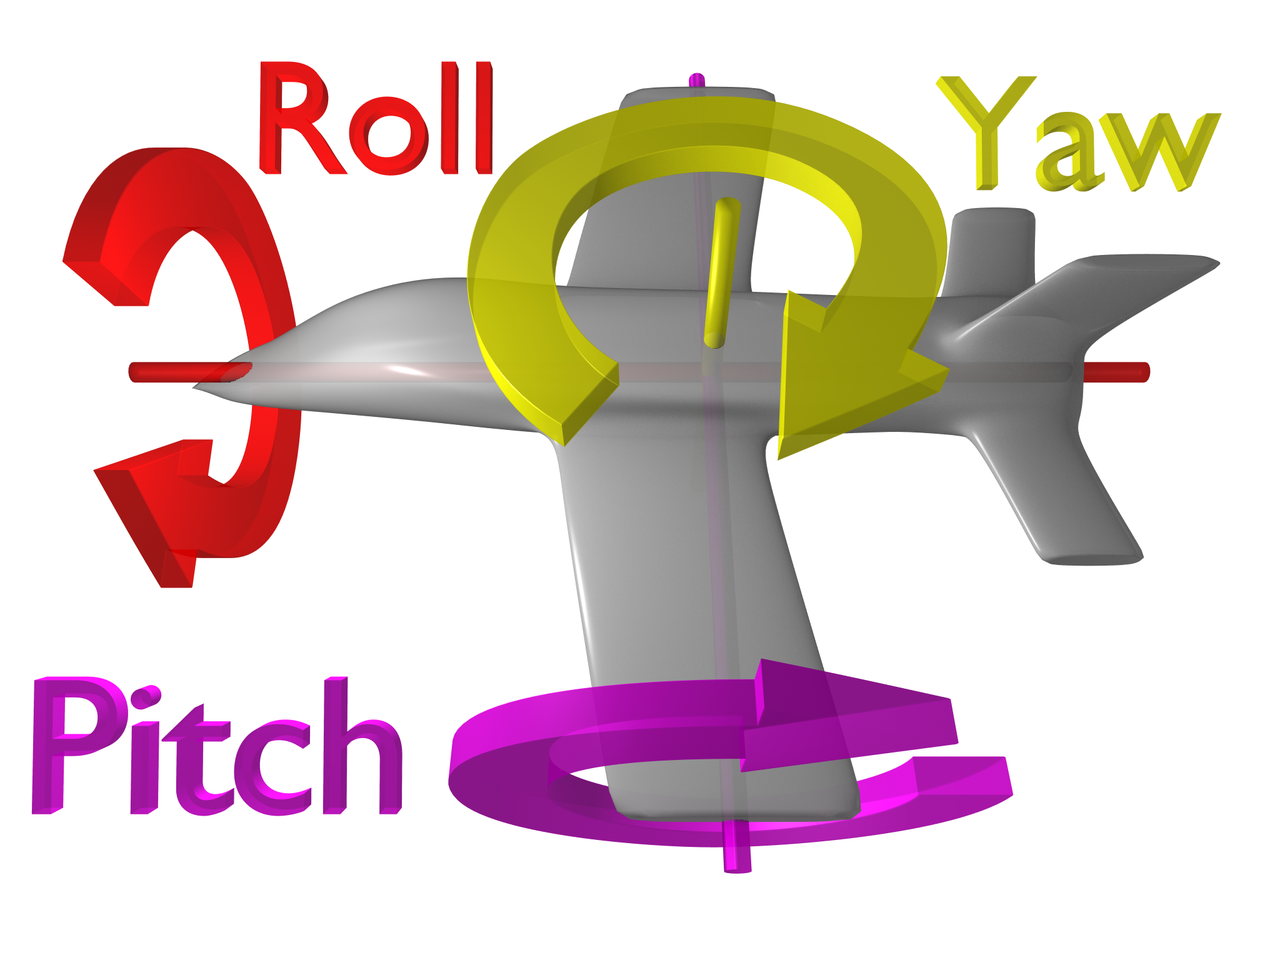
\includegraphics[width=0.55\textwidth]{img/airplane-axis}
        \caption{Pomenovanie osi otáčania.}
    \end{figure}

\end{frame}

\begin{frame}\frametitle{Použité knižnice}
    \begin{itemize}
        \item Extrakcia príznakov a predspracovanie obrazu - scikit-image, Keras
        \item Algoritmy strojového učenia - scikit-learn, Keras, TensorFlow
    \end{itemize}

    \vspace{0.4cm}

    \begin{figure}[H]
        \centering
        
\includegraphics[width=0.4\textwidth]{img/keras-tensorflow}
        %\caption{Pomenovanie osi otáčania.}
    \end{figure}

    \begin{figure}[H]
        \centering
        
\includegraphics[width=0.2\textwidth]{img/scikit-learn-logo}
        \qquad
        
\includegraphics[width=0.4\textwidth]{img/scikit-image-logo}
    \end{figure}

    %\begin{figure}[H]
     %   \centering
      %  
\includegraphics[width=0.4\textwidth]{img/scikit-image-logo}
        %\caption{Pomenovanie osi otáčania.}
    %\end{figure}
\end{frame}

% Frame
\begin{frame}\frametitle{Výsledky}
    \begin{table}
        \begin{tabular}{ l | c | c }
            \textbf{Typ klasifikácie}   & \textbf{Model}                    & \textbf{Presnosť}   \\
            \hline
            \textit{Krátke/Dlhé}    &                                   & {83,14 \%}           \\
            \textit{Pitch}          &                                   & {85,14 \%}           \\
            \textit{Roll}           &                                   & {91,02 \%}           \\
            \textit{Yaw}            & \multirow{-4}{*}{AlexNetLike}     & {49,71 \%}
        \end{tabular}
        \caption{Výsledna presnosť modelov.}
    \end{table}

    

\end{frame}

\begin{frame}\frametitle{Príklad klasifikácie}
    \begin{figure}[H]
        \centering
        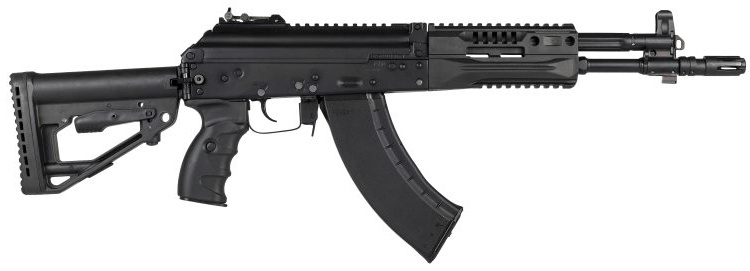
\includegraphics[width=0.5\textwidth]{img/prediction-weapon}
        
\includegraphics[width=0.9\textwidth]{img/result-prediction}
        \caption{Príklad správneho výsledku klasifikácie.}
    \end{figure}

    \begin{figure}[H]
        \centering
        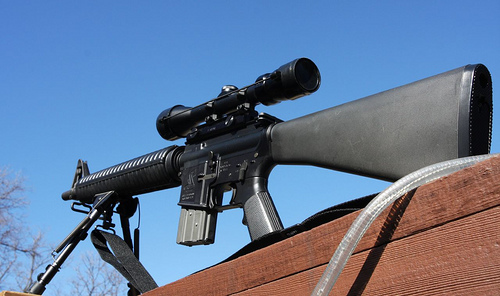
\includegraphics[width=0.4\textwidth]{img/weapon_2023}
        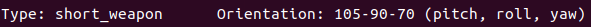
\includegraphics[width=0.9\textwidth]{img/class_bad}
        \caption{Príklad nesprávneho výsledku klasifikácie.}
    \end{figure}

\end{frame}

\appendix

% Last page
\bluepage{Ďakujem za pozornosť.}

% Questions
\addtocounter{framenumber}{-\value{framenumber}} % Framennumber reset

\begin{frame}
\frametitle{1. Otázka oponenta}
    Z jakého důvodu je testovací množina pro hodnocení úspěšnosti neuronových sítí menší oproti množině pro testování detektoru založeného na SVM (Support Vector Machine)?
    \vspace{0.3cm}
    \begin{itemize}
        \item SVM, 1 cyklus, 5-násobene dáta augmentáciou,
        \item 1,700 * 5 = 8,500 obrázkov (5,950 trénovanie, 2,550 testovanie).
        \vspace{0.2cm}
        \item CNN, \textit{n} cyklov, augmentácia pre každý cyklus,
        \item 1,700 obrázkov (1,190 trénovanie, 255 validácia, 255 testovanie).
    \end{itemize}
\end{frame}

\begin{frame}
\frametitle{2. Otázka oponenta}
    Jaké jsou další možnosti pro zlepšení detekce zbraní v obraze?
    \vspace{0.3cm}
    \begin{itemize}
        \item Kvalitnejšie a väčšia variácia 3D modelov pre generovanie vstupných dát.
        \item Väčšie množstvo vstupných dát.
        \item Použiť už natrénovane modely hlbokých CNN.
    \end{itemize}
\end{frame}

\end{document}
